\section{Petri Nets}\label{sec_pn_basic}

% ***************** Petri Net Basics ********************
A \emph{Petri net} is a 4-tuple $N=(P,T,W,M_N)$ where
$P$ is a finite set of \emph{places} and $T$ is a finite set of \emph{transitions}
with $P \cap T=\emptyset$,
$W: P\times T \cup T \times P \rightarrow \nat_0$ is the \emph{weight function,} and
$M_N$ is the \emph{initial marking}, where a \emph{marking} is a multiset of places,
\ie a function $P\rar\nat_0$ which assigns a number of \emph{tokens} to each place.
A Petri net can be considered as a bipartite graph with weighted arcs between places and transitions.
If necessary, we write $P_N$ etc.\ for the components of $N$ or $P'$ ($P_i$) etc.\ for the net $N'$ ($N_i$) etc.


% ***************** Preset, Postset ********************

The \emph{preset} of a place or transition $x$ is denoted as $\pre x$ and defined by
$\pre x\DEF\{y\in P\cup T\ |\  W(y,x)>0\}$,
the \emph{postset} of $x$ is denoted as $\post x$ and defined by
$\post x\DEF\{y\in P\cup T\ |\ W(x,y)>0\}$.
These notions are extended to sets as usual.
We say that there is an \emph{arc}
from each $y\in \pre x$ to~$x$.




% ***************** Enabledness, Reachable States ********************

A transition $t$ is \emph{enabled under a marking M}
if $\forall p\in \pre t:M(p)\geq W(p, t)$, which is denoted by $M\tfrs t$.
An enabled transition $t$ can \emph{fire} yielding a new marking $M'$,
written as $M\tfrs t M'$,
where $M'(p)=M(p)-W(p, t) + W(t,p)$, for all $p\in P$.
A transition sequence $\sigma=t_1\ldots t_n$ is \emph{enabled under a marking $M$} (yielding $M'$)
if $M\tfrs{t_1}M_1\tfrs{t_2}\ldots M_{n-1}\tfrs {t_n} M_n=M'$, and we
write $M\tfrs \sigma$, $M\tfrs \sigma M'$ resp.; $\sigma$ is called \emph{execution of $N$} if $M_N\tfrs \sigma$.
  The empty transition sequence $\lambda$ is  enabled under every marking.
$M$ is called \emph{reachable} if a transition sequence $\sigma$ with
$M_N\tfrs \sigma M$ exists.

$N$ is called \emph{bounded} if, for every reachable marking $M$ and every place $p$, $M(p)\leq k$ for some constant $k\in \nat$; if $k=1$, $N$ is called \emph{safe}. $N$ is bounded if and only if the set $\tfrs {M_N}$ of reachable markings is finite. In this thesis, we are mostly concerned with bounded Petri nets.

A place $p$ is \emph{implicit} if it can be deleted from the net
without changing the set of executions, and so an implicit place can be removed from the net without affecting its behaviour.\footnote{Note that an implicit place can cease to be implicit if another implicit place is removed first.}
Unfortunately, detecting
implicit places is expensive: the problem is \PSPACE-complete for safe and \EXPSPACE-complete for general Petri nets. A place $p$ is \emph{duplicate} if there is another place $p'$ with the same pre- and postsets whose initial marking does not exceed that of $p$. Duplicate places are implicit, and are cheap to detect.

\smallskip

An \emph{STG} is a tuple $N=(P,T,W,M_N,\I,\Ot,\ell)$ where
$(P,T,W,M_N)$ is a Petri net and $\I$ and $\Ot$  are disjoint
sets of \emph{input} and  \emph{output signals}. For
$\Sig=\I\cup\Ot$ being the set of all signals,
$\ell:T\rightarrow\Sig\times\{+,-\}\cup \{\lambda\}$ is the
\emph{labelling} function. $\Sig\times\{+,-\}$ or short
$\Sig\upd$ is the set of \emph{signal transitions}; its
elements are denoted  as $s^+$, $s^-$  resp.\ instead of
$(s,+)$, $(s,-)$ resp. A plus sign denotes that a signal value
changes from \emph{logical low} (written as 0) to \emph{logical
high} (written as 1), and a minus sign denotes the opposite
direction. We write $s\upd$ if it is not important or unknown
which direction takes place.

An STG can contain transitions labelled with $\lambda$, called
\emph{dummy} transitions, which do not correspond to any signal
change. \emph{Hiding a signal $s$} means to change the label of
all transitions labelled with $s\upd$ to $\lambda$. (The idea
of re-synthesis approach is to hide the signals used for
communication between components, which results in an STG with
fewer signals that often has a simpler implementation as a
circuit.) The labelling of an STG is called \emph{injective} if
for each pair of distinct non-dummy transitions $t$ and $t'$,
$\ell(t)\neq\ell(t')$.

\smallskip

Examples of STGs are shown in Figs.~\ref{fi-motivating-example1} and~\ref{fi-motivating-example2}.
Places are drawn as circles containing a number of tokens corresponding to the initial marking.
Unmarked places which have only one transition in their presets and postsets are
not drawn if the corresponding arcs have the weight~1; they are implicitly
given by an arc between these two transitions (and if such a place contains tokens, they are drawn on the arc itself). Transitions are drawn simply as their labels,
and the weight function is drawn as directed arcs $(x,y)$ whenever $W(x,y)\neq 0$ (and
labelled with $W(x,y)$ if $W(x,y)>1$).


\smallskip

% ********************** labels ***************************

We lift the notion of enabledness to transition labels: we write
$M\ifrs {\ell(t)}  M'$ if $M\tfrs t  M'$. This is extended to sequences
as usual -- deleting $\lambda$-labels automatically since $\lambda$
is the empty word; \ie $M\ifrs{s\upd}M'$ means that a sequence of
transitions fires, where one of them is labelled $s\upd$ while the
others (if any) are $\lambda$-labelled. A sequence
$\nu\in(\Sig\upd)^*$ is called a \emph{trace of a marking} $M$ if
$M\ifrs \nu$, and a \emph{trace} of $N$ if $M=M_N$. The \emph{language $L(N)$
of $N$} is the set of all traces of $N$.

\smallskip

The \emph{reachability graph} $\RG(N)$ of an STG $N$ is an arc-labelled
directed graph on the reachable markings of $N$ with $M_N$ as the root;
there is an arc from $M$ to $M'$ labelled $\ell(t)$ whenever
$M\tfrs {t} M'$. For bounded Petri nets and STGs, $\RG(N)$ can be seen as a finite automaton
(where all states are accepting), and $L(N)$ is the language of this
automaton.
Observe that automata with accepting states only can be
regarded as STGs (with the states as places, the initial state being the
only marked place, etc.); hence, all definitions for STGs also
apply to automata.

$N$ is \emph{deterministic} if $\RG(N)$
is a deterministic automaton: it contains no $\lambda$-labelled transitions
and there are no \emph{dynamic auto-conflicts,} \ie for each reachable marking $M$ and each signal transition $s\upd$
there is at most one $M'$ with $M \ifrs {s\upd} M'$. (Note that a deterministic STG
can have choices between different outputs, \eg an STG modelling
the standard arbiter is deterministic).

An STG with a set of all markings $S_2$ is said to \emph{simulate} another STG with 
a set of all markings $S_1$ iff there exist an 
$R \subset S_1 \times S_2$ such that $(M_{N 1},M_{N 2}) \in R$ and for any pair of markings 
$(M_1, M_2) \in R$, a label $l$ and a marking $M_1'$, $M_1\ifrs {l}  M_1'$ implies 
$M_2 \ifrs {l} M_2'$ for some $M_2'$. We call $R$ the witness of simulation. Now we can say that STGs $N_1$ and $N_2$ are \emph{bisimilar} iff $N_2$ simulates $N_1$ with witness $R$ and $N_2$ simulates $N_1$ with witness $R^{-1}$.

For deterministic STGs, language equivalence and bisimulation coincide, and the language can be taken as the semantics of such a specification. Unfortunately, the class of deterministic STGs is too restrictive in practice~\cite{KSV-08}, \eg:
\begin{itemize}
  \item using dummy transitions is often convenient in manual design;
  \item modelling OR-causality~\cite{ykklp96} as a safe STG requires non-determinism;
  \item hiding internal communication (and thus introducing dummy transitions) is a crucial step in re-synthesis.
\end{itemize}
Hence, one has to deal with non-deterministic STGs as well.

One might think that if $\RG(N)$ is non-deterministic, it can be \emph{determinised} (using well-known auto\-ma\-ta-the\-o\-re\-tic methods), \ie turned  into a language-equivalent deterministic
automaton with accepting states only; in particular, the resulting automaton will have no $\lambda$-arcs. Unfortunately, this is a bad idea, as shown in~\cite{KSV-08}, where the semantics of non-deterministic STGs was developed. It is based on the concept of \emph{output-determinacy,} which is a relaxation of determinism: An STG $N$ is \emph{output-determinate (OD)} if $M_N \ifrs {\nu}
M_1$ and $M_N \ifrs {\nu} M_2$ implies for every $x\in \Ot_N$ that
$M_1 \ifrs {x\upd}$ iff $M_2 \ifrs {x\upd}$.
It turns out that OD STGs are exactly the STGs which
have correct implementations according to the implementation relation introduced in~\cite{KSV-08}.
Hence, non-OD STGs are ill-formed, and in particular cannot be correctly implemented as
circuits. This shows that in general, \emph{the language is not a satisfactory semantics of
non-deterministic STGs;} in particular, \emph{synthesising the determinised reachability graph of a non-OD STG
will either fail or result in an incorrect circuit.} On the other hand, for the class of OD STGs~\cite{KSV-08} shows that their language
is an adequate semantics, and
implementation relation can be formulated purely in terms of the language.
An important property of OD STGs is that in them the enabledness of an output signal is a function of the trace, \ie given a trace $\nu$, the set of outputs by which $\nu$ can be extended is uniquely determined, even though there could be multiple executions corresponding to $\nu$.


\smallskip

In the following definition
of {\em parallel composition}~$\parallel$, see \eg~\cite{vowo02lncs}, we will have to
consider the distinction between input and output signals.
The idea of parallel composition is that the
composed systems run in parallel and synchronise on common actions
-- corresponding to circuits that are connected on the
wires corresponding to the signals.
Since a system controls its outputs, we cannot allow a signal to
be an output of more than one component; input signals, on the other
hand, can be shared.
An output signal of a component may be an input of
other components, and in any case it is an output of the composition.

The parallel composition of STGs $N_1$ and $N_2$ is defined if
$\Ot_1 \cap \Ot_2 = \emptyset$. If we drop this requirement, the
definition gives the {\em synchronous product} $N_1\times N_2$,
which is often useful. The place set of the composition is
the disjoint union of the place sets of the components; therefore,
we can consider markings of the composition (regarded as multisets)
as the disjoint union of markings of the components,
and we will also write such a marking $M_1 \dot{\cup} M_2$
of the composition as $(M_1, M_2)$. To define the transitions,  let
$A=(\I_1 \cup \Ot_1) \cap (\I_2 \cup \Ot_2)$ be the set of
common signals.
If \eg $s$ is an output of $N_1$ and an input of $N_2$,
then firing of $s\upd$ in $N_1$ is `seen' by
$N_2$, \ie it must be accompanied by firing of $s\upd$
in $N_2$. Since we do not know a priori which $s\upd$-labelled
transition of $N_2$ will fire together with some $s\upd$-labelled
transition of $N_1$, we have to allow for each possible
pairing.
Thus, the {\em parallel composition} $N = N_1 \parallel N_2$
is obtained from the disjoint union of $N_1$ and $N_2$ by
fusing
each $s\upd$-labelled transition $t_1$ of $N_1$
with each $s\upd$-labelled transition $t_2$ from $N_2$ if $s \in A$.
Such transitions are pairs and the firing $(M_1, M_2)\tfrs{(t_1,t_2) }(M_1', M_2')$ of $N$
corresponds to the firings $M_i\tfrs{t_i}M_i'$ in $N_i$, $i=1,2$; for an example
of a parallel composition, see Fig.~\ref{fig_parcom}.
More generally, we have $(M_1, M_2) \ifrs{\nu} (M_1', M_2')$ iff
$M_i \ifrs{\nu|_{N_i}} M_i'$ for  $i\in\{1,2\}$, where
$\nu|_{N_i}$ denotes the projection of the trace $\nu$ onto the signals of the STG ${N_i}$.
Hence, all reachable markings of $N$ have the form $(M_1, M_2)$,
where $M_i$ is a reachable marking of $N_i$, $i=1,2$.

Obviously, one can extend the notion of the parallel
composition to a finite family (or collection) $(C_i)_{i\in I}$ of
STGs as $\parallel_{i\in I} C_i$,
provided that no signal is an output signal of more than one of the
$C_i$. We will also denote the markings of such a composition
by $(M_1, \ldots,M_n)$ if $M_i$ is a marking of $C_i$ for
$i\in I=\{1,...,n\}$.
As above, $(M_1, M_2, \ldots, M_n) \ifrs{\nu} (M_1', M_2', \ldots, M_n')$ iff
$M_i \ifrs{\nu|_{C_i}} M_i'$ for all $i\in\{1,\ldots,n\}$.
It is easy to see that $C$ is deterministic if all $C_i$ are. However, this is not true for a composition of OD STGs, as the result, in general, can be non-OD in such a case.

A composition can also be ill-defined due to \emph{computation interference,} see \eg~\cite{eber92}.
Let $C\DEF\parallel_{i\in I}C_{i}$ be a composition of STGs. It is
\emph{free from computation interference (FCI)} if for every trace $\nu$ of $C$
the following holds: if $\nu|_{C_{j}}x^{\pm}$ is a trace of $C_{j}$
for some output $x$ of $C_{j}$, then $\nu|_{C}x^{\pm}$ is a trace
of $C$.

\begin{figure*}[t]
    \centering
    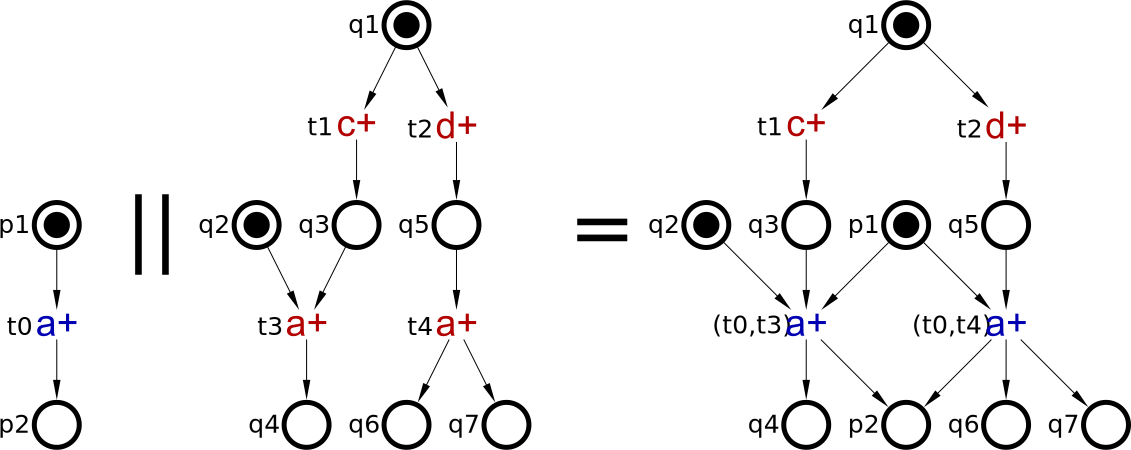
\includegraphics[scale=0.4]{EXPERIMENTS/stg/pcomp_example}
    \caption{\label{fig_parcom}
        Parallel composition example. In the net fragment on the left hand side,
        signal $a$ is an output, and in the fragment in the middle it is an input.
        Hence, in their parallel composition (right) it is an output.
        In this example, there is \emph{computation interference}: the left component activates $a\up$ but the middle one is not ready to receive it.}
\end{figure*}

\smallskip


\begin{figure*}[!tb]
    \centering
    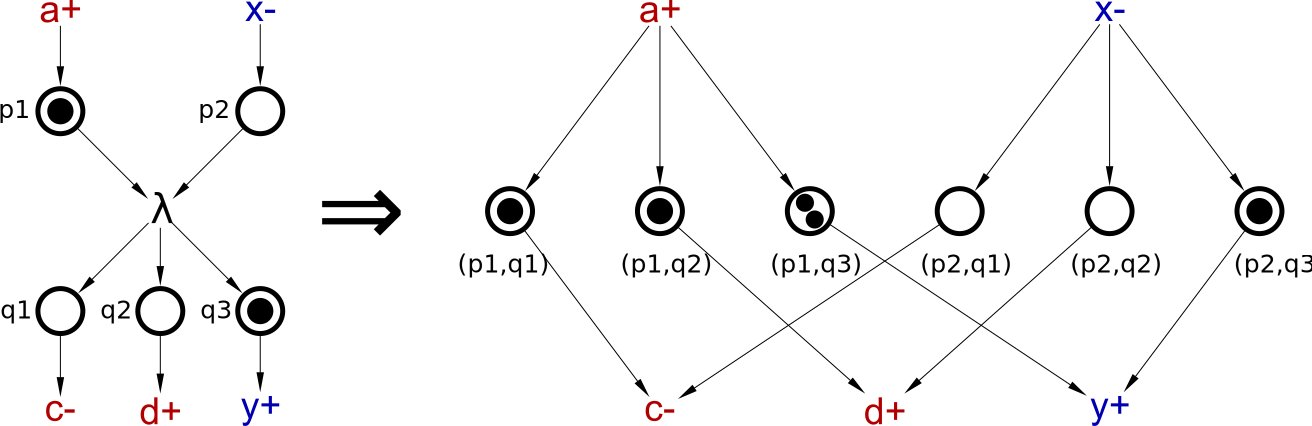
\includegraphics[scale=0.4]{EXPERIMENTS/stg/transition_contraction}
    \caption{\label{fig3.1}
        An example of a transition contraction.
    }
\end{figure*}


\emph{Transition contraction}~\cite{vowo02lncs} is an important operation in circuit re-synthesis. It removes a dummy transition from an STG and
combines each place of its preset with each place of its postset to `simulate' the
firing of the deleted transition, see Fig.~\ref{fig3.1}. Unfortunately, transition contractions are sometimes undefined (\eg in case the transition has a self-loop, \ie some place occurs in both its preset and postset); moreover, even when a contraction is defined, it might change the semantics of the STG.
Hence,~\cite{vowo02lncs} uses the notion of \emph{secure} contractions, that preserve the semantics.

Transition contractions preserve boundedness, but in general,
can turn a safe net into a non-safe one, as well as
introduce weighted arcs. In practice, it is often convenient to work with safe nets, and for this~\cite{KSVW-09} introduced \emph{safeness-preserving} contractions, \ie ones which
guarantee that  the transformed STG is safe if the initial one
was. (Note that the transitions with weighted arcs must be dead
in a safe Petri net, and so we can assume that the initial and
all the intermediate STGs contain no such arcs.) Also,~\cite{KSVW-09} developed a sufficient structural
condition for a contraction to be safe\-ness-pre\-ser\-ving.

From the point of view of this thesis, it is important to remark that implicit places can adversely affect the (secure) contractibility of a transition, \ie it is possible to have a situation when a transition is not contractible (or not securely contractible), but becomes securely contractible after some implicit place is removed from the STG. As detecting implicit places is expensive, it is very desirable to reduce their number by some other means, in particular the approach proposed in this thesis reduces the number of such places in STGs obtained by parallel composition. This has a direct effect on re-synthesis: if the composed STG has fewer implicit places, more dummy transitions in it can be contracted, and so it will be easier to synthesise the result.
